\chapter{Tömbképletek a Calcban}
\thispagestyle{empty}

\section{Tömbképletek létrehozása}

A Calcban megoldatjuk, hogy egy képletet beírva az eredményül
több cellának is értéket adjon. Az ilyen képletet
tömbképletnek nevezzük. Tömbnek értékeket tartalmazó
cellák kapcsolt tartományát nevezzük. A tömb sorokból és
oszlopokból áll. Egy 4 sorból és 3 oszlopból álló
tömböt 4-szer 3-as tömbnek nevezünk. A 4 és a 3 a tömb
dimenziói. A tömb dimenzióit mindig először a sorok
számával, majd az oszlopok számával adják meg.

A tömbökkel való munkát megkönnyíti, ha a tömbök
cellatartományait nevekkel határozzuk meg.

Tömbképletet úgy hozunk létre, hogy kijelöljük azt a
tartományt, amelyik celláit tömbképlettel akarunk feltölteni,
beírjuk a képletet, majd a Shift+Ctrl+Enter
billentyűkombinációt ütjük le.

A függvénytündér segítségével is létrehozhatunk
tömbképletet, ha bekapcsoljuk az \textbf{Adattömb} kapcsolót az
ablak bal alsó sarkában. 

A tömbök celláiba számokat írva a matematikából ismert
mátrixokat kapunk. A mátrixokat nagybetűvel jelölik és
elemeit szögletes zárójelek közé írják. Mátrixokat
használnak lineáris egyenletek leírására és olyan adatok
tárolására amelyek két paramétertől függnek.


\section{Mátrixok összeadása}

Két mátrixot úgy adunk össze, hogy a megfelelő elemeit
összeadjuk. Hozzunk létre \aref{MátrixokÖsszeadásaNevek} ábrán látható
A és B mátrixokat. A B2:D4 tartomány neve legyen \textbf{Atömb}, az
F2:H4 tartományé pedig \textbf{Btömb}.

\begin{figure}[!h]
\begin{center}
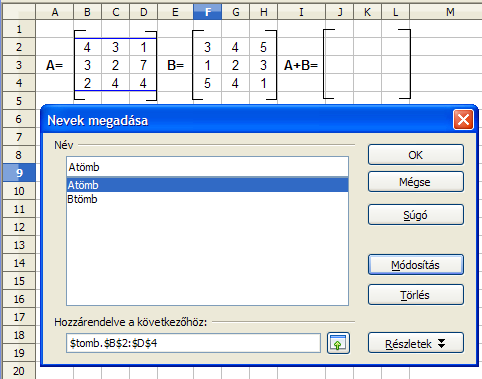
\includegraphics[width=12.751cm]{oocalcv1-img130.png}
\caption{Mátrixok összeadása -- Nevek megadása}\label{MátrixokÖsszeadásaNevek}
\end{center}
\end{figure}

A szögletes zárójeleket megrajzolhatjuk a \textbf{Rajz}
eszköztárt bekapcsolva, azon a \textbf{Szimbolikus alakzatok
Nyitó zárójel} és \textbf{Záró zárójel} objektumokat választva.

Jelöljük ki a J2:L4 tartományt és írjuk be a következő
kifelezést: {\sffamily\bfseries{=Atömb+Btömb}}.

A kifejezés beírása után ne az Enter billentyűt, hanem a
Shift+Ctrl+Enter billentyűkombinációt üssük le. A
cellatartományban megjelennek az értékek, tömbképletet
hoztunk létre. Bármelyik cellát is választva a J2:L4
tartományból a következő tartalmat látjuk:
\{=Atömb+Btömb\} (\ref{MátrixokÖsszeadása} ábra).

\begin{figure}[!h]
\begin{center}
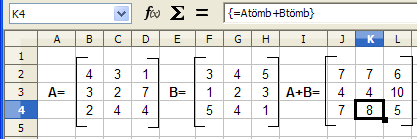
\includegraphics[width=10.031cm]{oocalcv1-img131.png}
\caption{Mátrixok összeadása}\label{MátrixokÖsszeadása}
\end{center}
\end{figure}

Ezek tömbhivatkozások, amit a Calc mindig kapcsos zárójelben
mutat. A kapcsos zárójelek kézi beírásával tömbképletet
nem hozhatunk létre.


\section{Mátrix szorzata skalárral}

Egy mátrix skalárral való szorzatát úgy számítjuk ki, hogy
a skalárral a mátrix minden elemét megszorozzuk. A
következő munkalapon számítsuk ki az \textbf{A} mátrix 3-al
való szorzatát. A B2:D4 tartomány kijelölése után írjuk
be a képletet majd a Shift+Ctrl+Enter billentyűkombinációval
érvényesítsük a tömbképletet (\ref{MátrixSzorzataSkalárral} ábra)

\begin{figure}[!h]
\begin{center}
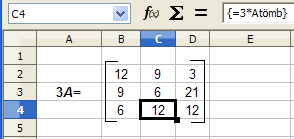
\includegraphics[width=7.077cm]{oocalcv1-img132.png}
\caption{Mátrix szorzata skalárral}\label{MátrixSzorzataSkalárral}
\end{center}
\end{figure}


\section{Mátrixok szorzása}

Két mátrixot csak akkor lehet összeszorozni, ha a baloldali
mátrix oszlopainak száma megegyezik a jobboldali mátrix sorainak
számával. A szorzat egy olyan mátrix lesz, amelyiknek annyi sora
van mint a baloldalinak és annyi oszlopa mint a jobboldalinak. A
mátrix elemeit az \textbf{Adattömb} kategóriában lévő
\textbf{MMULT} tömbfüggvénnyel számíthatjuk ki.

\Aref{MátrixokSzorzásaMMULT} ábrán a \textbf{C} és a \textbf{D}
mátrixok dimenziói
5x3 és 3x4, ami megfelel a feltételnek. A mátrixok ebben a
sorrendben összeszorozhatóak, más szóval konformábilisak. A
függvénytündér használata előtt vagy jelöljük ki
pontosan azt a tartományt, ahol az új mátrix sorai és oszlopai
lesznek, vagy az aktív cella legyen a leendő mátrix első
elemének a cellája. Hibás kijelölés esetén csak azt a
tartományt tölti fel értékekkel a tömbfüggvény.

\begin{figure}[!h]
\begin{center}
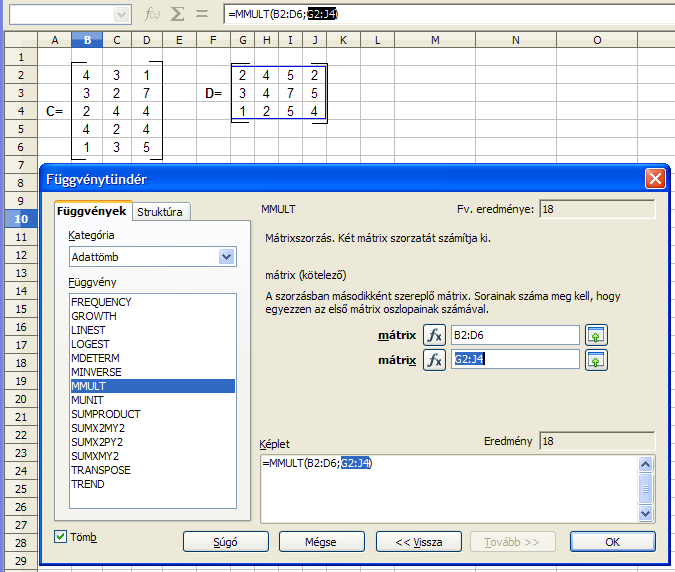
\includegraphics[width=13.999cm]{oocalcv1-img133.png}
\caption{Mátrixok szorzása -- MMULT függvény}\label{MátrixokSzorzásaMMULT}
\end{center}
\end{figure}

Az \textbf{Adattömb} kapcsoló automatikusan bekapcsol a függvény
használatakor. Az eredményt \aref{MátrixokSzorzásaEredmény} ábrán látjuk.

\begin{figure}[!h]
\begin{center}
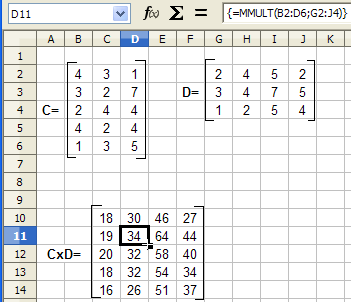
\includegraphics[width=8.285cm]{oocalcv1-img134.png}
\caption{Mátrixok szorzása -- eredmény}\label{MátrixokSzorzásaEredmény}
\end{center}
\end{figure}


\section[Mátrix determinánsának meghatározása]{Mátrix
determinánsának meghatározása}

A négyzetes mátrix determinánsát az \textbf{MDETERM}
függvénnyel számíthatjuk ki. Szintaxisa MDETERM(tömb).
Függvény nélkül, képlet segítségével nehézkes a
determináns meghatározása, hiszen a 3x3-as mátrix
determinánsa 6 tagból áll, a 4x4-es 24 tagból, a 6x6-os pedig
több mint 200-ból. 

\section{30. feladat}

{\itshape
Határozzuk meg a B2:D4 tartományba írt 3x3-as tömb
determinánsát képlet segítségével az F3 cellában, a
G3-ban pedig az MDETERM függvénnyel. A tömb számértékeinek
módosításával ellenőrizzük a determináns néhány
tulajdonságát:}

{\itshape
a) értékét megtartja, ha egyik sorának minden eleméhez
hozzáadjuk egy másik sor megfelelő elemeinek egy bizonyos m
számmal való szorzatát;}

{\itshape
b) értékét m-szeresére változtatja, ha egyik sorának elemeit
m-mel szorozzuk;}

{\itshape
c) csak előjelét váltja, ha két sorát felcseréljük;}

{\itshape
d) zérus, ha két sora megegyezik.}

A B2:D4 tartományba írt mátrix determinánsa a definíció
alapján a következő képlettel számítható ki:
{\sffamily\bfseries{=B2*C3*D4+C2*D3*B4+D2*B3*C4-B4*C3*D2-C4*D3*B2-D4*B3*C2 }}
(\ref{30-feladatMátrixMDETERM} ábra).
A G3 tartalma: {\sffamily\bfseries{=MDETERM(B2:D4)}}.

\begin{figure}[!h]
\begin{center}
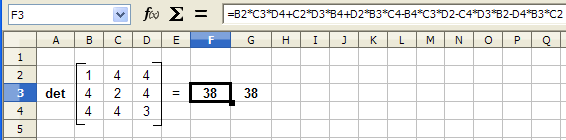
\includegraphics[width=12.974cm]{oocalcv1-img135.png}
\caption{30. feladat --  mátrix determinánsa --  MDETERM}\label{30-feladatMátrixMDETERM}
\end{center}
\end{figure}


\section{Mátrix inverze}

Egy mátrix inverzén olyan mátrixot értünk, amelynek szorzata a
mátrixszal egységmátrixot ad. Az egységmátrix olyan mátrix,
amelyik fő átlóján egyesek vannak minden más eleme pedig
nulla. Az \textbf{A} mátrix inverzét \textbf{A\textsuperscript{{}-1}}
szimbólummal jelöljük. Csak négyzetes mátrixoknak van inverzük.

A \textbf{MINVERSE} tömbfüggvénnyel határozhatjuk meg az inverz
mátrixot. Szintaxisa: MINVERSE(tömb). \Aref{MátrixInverse} ábrán a B2:D4
tartományba írt mátrix inverzét a B6:D8 tartományba
számítottuk ki a függvénnyel.

\begin{figure}[!h]
\begin{center}
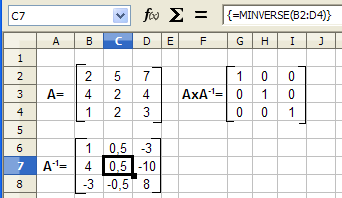
\includegraphics[width=8.047cm]{oocalcv1-img136.png}
\caption{Mátrix inverze --  MINVERSE}\label{MátrixInverse}
\end{center}
\end{figure}

A G1:I4 tartományban az ellenőrzést is elvégezhetjük.
Látható, hogy a mátrix és inverzének szorzata
egységmátrixot ad.


\section{Transzponált mátrix}
A \textbf{TRANSPOSE} tömbfüggvénnyel meghatározhatjuk egy
mátrix transzponáltját, olyan mátrixot amiben a sorok és az
oszlopok fel vannak cserélve. Szintaxisa: TRANSPONSE(tömb). 
\Aref{TranszponáltMátrix} ábrán a G2:I3 tartományba az
\textbf{A} tömb transzponáltját látjuk. 

\begin{figure}[!h]
\begin{center}
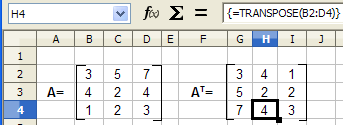
\includegraphics[width=8.073cm]{oocalcv1-img137.png}
\caption{Transzponált mátrix --  TRANSPOSE}\label{TranszponáltMátrix}
\end{center}
\end{figure}

Tömbképletet akkor is használhatunk, ha nem tartományt
töltünk fel képlettel, hanem egy konkrét cellában végzünk
számítást. A következő feladatban erre látunk példát.


\section{31. feladat}
{\itshape
\Aref{Adattartományok} ábrán látható adattartományban határozzuk meg,
hogy a következő értékhatárok között hány rekordot
találunk: 1--1~000~Ft; 1~000--10~000~Ft; 10~000--50~000~Ft;
50~000--200~000~Ft. Az alsó értékhatárt tekintsük szigorúnak.}

A feladat megoldásához másoljuk egy üres munkalapra az
adattáblát, és készítsük el az értékhatárok
táblázatát (\ref{31-feladat} ábra). 

\begin{figure}[!h]
\begin{center}
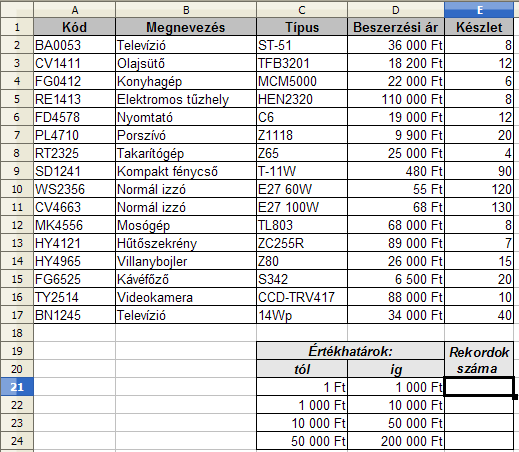
\includegraphics[width=10.73cm]{oocalcv1-img138.png}
\caption{31. feladat}\label{31-feladat}
\end{center}
\end{figure}

Az E21 cellában azt kell meghatározni, hogy hány olyan sora van az
adattartománynak ahol a beszerzési ár nagyobb, mint 1~Ft de
kisebb vagy egyenlő 1000~Ft-nál.

Írjuk be a következő kifejezést az E21 cellába:\\
{\sffamily\bfseries{=SUM(IF(D\$2:D\$17>C21;IF(D\$2:D\$17<=D21;1;0)))}}.

A képletet a Ctrl+Shift+Enter billentyűkombinációval
nyugtázzuk, tehát tömbképletet hozzunk létre. A
tömbképlet ebben az esetben megvizsgál minden cellát a D2:D17
tartományból és az egymásba ágyazott IF függvényeknek
köszönhetően 1-nek tekinti azokat értékeket, amelyek
megfelelnek a feltételeknek, és 0-nak ha nem. Ezeknek az összege
megadja a kívánt rekordszámot.

A tömbképlet másolásakor a Ctrl billentyűt lenyomva kell
tartani, hogy a Calc ne tömböt hozzon létre, hanem önálló
cellatartalmakat. A feladat megoldását \aref{31-feladatMegoldás}
ábrán látjuk.

\begin{figure}[!h]
\begin{center}
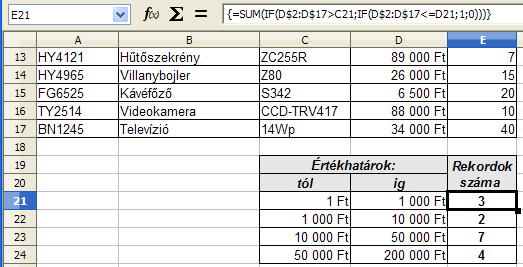
\includegraphics[width=11.834cm]{oocalcv1-img139.png}
\caption{31. feladat -- megoldás}\label{31-feladatMegoldás}
\end{center}
\end{figure}

Bár ezt a feladatot megoldhatjuk tömbképlet
alkalmazása nélkül is, például COUNTIF függvénnyel  a
\& operátort
felhasználva\footnote{=COUNTIF(D\$2:D\$17;"<"\&D21)-COUNTIF(D\$2:D\$17;"<"\&C21)},
de a fent bemutatott megoldás is tanulságos.

